\documentclass{standalone}
\usepackage{tikz}
\usepackage{mathdots}
\usetikzlibrary{matrix,decorations.pathreplacing, calc, positioning,fit}
\begin{document}
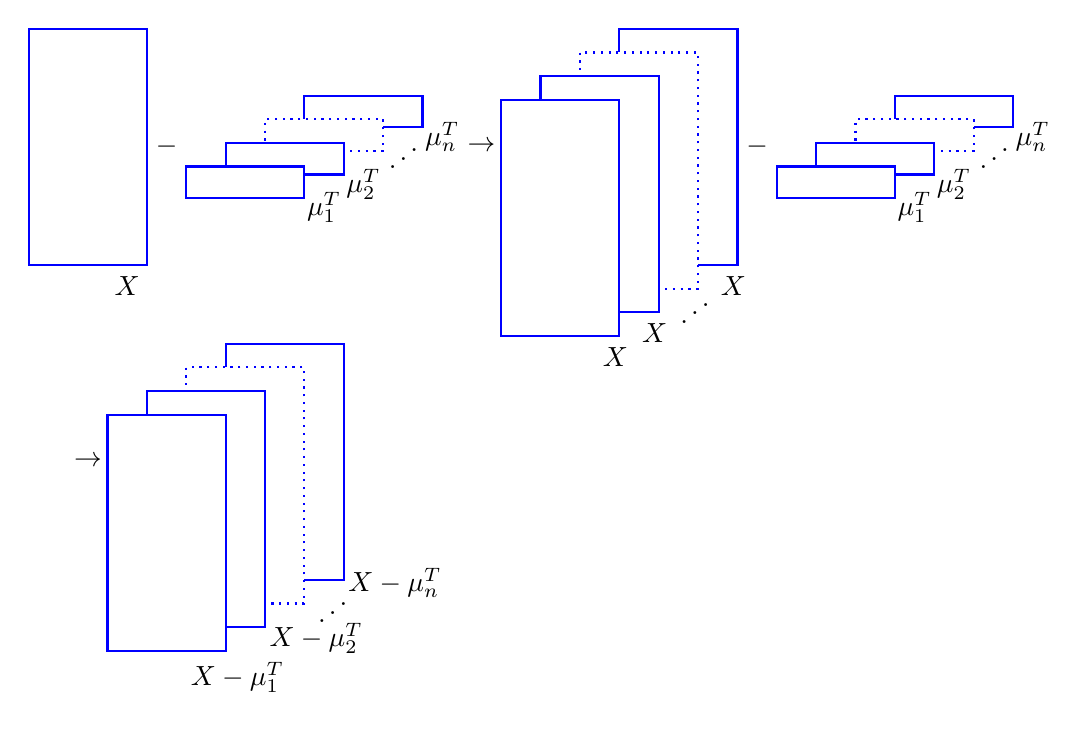
\begin{tikzpicture}[>=stealth,thick,baseline,
  mtxstyle/.style={
    draw=blue,
    minimum width=1.5cm,
    minimum height=3cm,
    inner sep=1pt,
    fill=white},
  vecstyle/.style={
    mtxstyle,
    minimum height=4mm}
    ]

% \tikzstyle{mxborder} = [matrix of mathnodes, draw, blue];
    \node (A) [mtxstyle] {};
   \node (Ax) [right=0.5cm of A.south, anchor=north] {$X$};
   \node (B) [right of = A] {$-$};
   \node (C) [right of = B, xshift=15mm, yshift=4.5mm, vecstyle] {};
   \node (Cm) [right of = C, anchor=north] {$\mu_n^T$};
   \node (C2) [right of = B, xshift=10mm, yshift=1.5mm, vecstyle, dotted] {};
   \node (C2m) [right of = C2, yshift=2mm, anchor=north] {$\iddots$};
   \node (C3) [right of = B, xshift=5mm, yshift=-1.5mm, vecstyle] {};
   \node (C3m) [right of = C3, anchor=north] {$\mu_2^T$};
   \node (C4) [right of = B, xshift=0mm, yshift=-4.5mm, vecstyle] {};
   \node (C4m) [right of = C4, anchor=north] {$\mu_1^T$};
   \node (D) [right of = B, xshift=3cm] {$\rightarrow$};

  \node (E) [right of= D, xshift=15mm, mtxstyle] {};
   \node (Em) [right=0.7cm of E.south, anchor=north] {$X$};
  \node (E1) [right of= D, xshift=10mm, yshift=-3mm, mtxstyle, dotted] {};
   \node (E1m) [right=0.7cm of E1.south, yshift=2mm, anchor=north] {$\iddots$};
  \node (E2) [right of= D, xshift=5mm, yshift=-6mm, mtxstyle] {};
   \node (E2m) [right=0.7cm of E2.south, anchor=north] {$X$};
  \node (E3) [right of= D, xshift=0mm, yshift=-9mm, mtxstyle] {};
   \node (E3m) [right=0.7cm of E3.south, anchor=north] {$X$};
   \node (F) [right of = E] {$-$};
   \node (G) [right of = F, xshift=15mm, yshift=4.5mm, vecstyle] {};
   \node (Gm) [right of = G, anchor=north] {$\mu_n^T$};
   \node (G2) [right of = F, xshift=10mm, yshift=1.5mm, vecstyle, dotted] {};
   \node (G2m) [right of = G2, yshift=2mm, anchor=north] {$\iddots$};
   \node (G3) [right of = F, xshift=5mm, yshift=-1.5mm, vecstyle] {};
   \node (G3m) [right of = G3, anchor=north] {$\mu_2^T$};
   \node (G4) [right of = F, xshift=0mm, yshift=-4.5mm, vecstyle] {};
   \node (G4m) [right of = G4, anchor=north] {$\mu_1^T$};

   \node (H) [below of = A, yshift=-3cm] {$\rightarrow$};
  \node (J) [right of= H, xshift=15mm, mtxstyle] {};
   \node (Jm) [right=1.4cm of J.south, yshift=3mm, anchor=north] {$X - \mu_n^T$};
  \node (J1) [right of= H, xshift=10mm, yshift=-3mm, mtxstyle, dotted] {};
   \node (J1m) [right=1.1cm of J1.south, yshift=4mm, anchor=north] {$\iddots$};
  \node (J2) [right of= H, xshift=5mm, yshift=-6mm, mtxstyle] {};
   \node (J2m) [right=1.4cm of J2.south, yshift=2mm, anchor=north] {$X - \mu_2^T$};
  \node (J3) [right of= H, xshift=0mm, yshift=-9mm, mtxstyle] {};
   \node (J3m) [right=0.9cm of J3.south, anchor=north] {$X - \mu_1^T$};

\end{tikzpicture}
\end{document}